\section{Numerical method for chemical equilibrium calculation}
%
% --------------------------------------------------------------------------------------------------------------------%
% Recap of a chemical equilibrium problem
% --------------------------------------------------------------------------------------------------------------------%
%
\begin{frame}{Recap of a chemical equilibrium problem}

\lcol
\begin{itemize}
\item Calculate the amounts of the species in each phase at equilibrium
at given:
\begin{itemize}
\item \textbf{temperature} (e.g., 100 ~ °C);
\item \textbf{pressure} (e.g, 300 bar); and 
\item \textbf{amounts of elements H, O, C, Na, Cl} 
\item \textbf{Note}: the latter is rather given as a recipe that determine the values of H, O, C, Na, Cl by formula matrix b = A n, e.g., 
\begin{itemize}
\item 1 kg of H$_{2}$O,
\item 1 mol CO$_{2}$, 
\item 0.1 mol of NaCl.
\end{itemize}
% 

\end{itemize}
\end{itemize}
\rcol
\begin{center}
\begin{table}
\centering
\scriptsize%
\begin{tabular}{ccc}
\toprule 
\multicolumn{1}{c}{\textbf{Aqueous Phase}} & \textbf{Gaseous Phase} & \textbf{Mineral Phases}\tabularnewline
\midrule
H$_{2}$O(aq) & CO$_{2}$(g) & NaCl(s, halite)\tabularnewline
H$^{+}$(aq) & H$_{2}$O(g) & \tabularnewline
OH$^{-}$(aq) &  & \tabularnewline
Na$^{+}$(aq) &  & \tabularnewline
Cl$^{-}$(aq) &  & \tabularnewline
\multicolumn{1}{c}{CO$_{2}$(aq)} &  & \tabularnewline
HCO$_{3}^{-}$(aq) &  & \tabularnewline
\multicolumn{1}{c}{CO$_{3}^{2-}$(aq)} &  & \tabularnewline
\bottomrule
\end{tabular}
\end{table}
\par\end{center}

\ecol
\end{frame}
% --------------------------------------------------------------------------------------------------------------------%
% Chemical equilibrium equations, Fundamental condition
% --------------------------------------------------------------------------------------------------------------------%
%
\begin{frame}{Chemical equilibrium equations, Fundamental condition}

\alert{\textbf{Fundamental condition for chemical equilibrium}} reads as follows:
\vskip 5pt
%
\begin{cbox}{Gibbs energy minimization (GEM) problem}

Given temperature $T$, pressure $P$, and elements amounts ${b=(b_{1},\ldots,b_{\text{E}})}$,
find the amounts of the species ${n=(n_{1},\ldots,n_{\text{N}})}$
that solve the \textbf{constrained minimization problem}:
\[
\min_{n}G(n)\qquad\text{subject to (s.t.)}\qquad An=b\quad\text{and}\quad n\geq0.
\]

\end{cbox}
\vskip 5pt
%
\begin{center}
How do we transform it into a system of equations from which species amounts $n=(n_{1},\ldots,n_{\text{N}})$ can be calculated?
\end{center}

\end{frame}
% --------------------------------------------------------------------------------------------------------------------%
% Chemical equilibrium equations, Finding the minimum
% --------------------------------------------------------------------------------------------------------------------%
%
\subsection{Unconstrained minimization}
%
\begin{frame}{Chemical equilibrium equations, Finding the minimum}

\small
\begin{itemize}[<+->]
\item Assume there were \textbf{no constraints} of mass conservation and non-negative bounds.
%\[
%An=b\qquad\text{and}\qquad n\geq0.
%\]
%
\item Then, the \alert{\textbf{chemical equilibrium equations}} would result from
the condition
\[
\frac{\partial G}{\partial n_{i}}=0\qquad(i=1,\ldots,\text{N}),
\]
%
which corresponds to a state in which the {\bf Gibbs energy does not change with infinitesimal changes in the amounts of the species}. 
%
\item {\bf But!} some care would still be needed to ensure that a \textbf{minimum is found}, and not a \alert{\bf maximum} or \alert{\bf saddle point}.
\end{itemize}
\end{frame}
%
% --------------------------------------------------------------------------------------------------------------------%
% Example of minimization problem
% --------------------------------------------------------------------------------------------------------------------%
%
\begin{frame}{Example of finding the minimum}
\small
\begin{columns}[t]
	
\column{0.4\textwidth}
\vskip 20pt
\begin{itemize}
\item Consider the function $f$ defined as:
\[
f(x,y)=(x-1)^{2}+(y+1)^{2}.
\]
\vskip -5pt
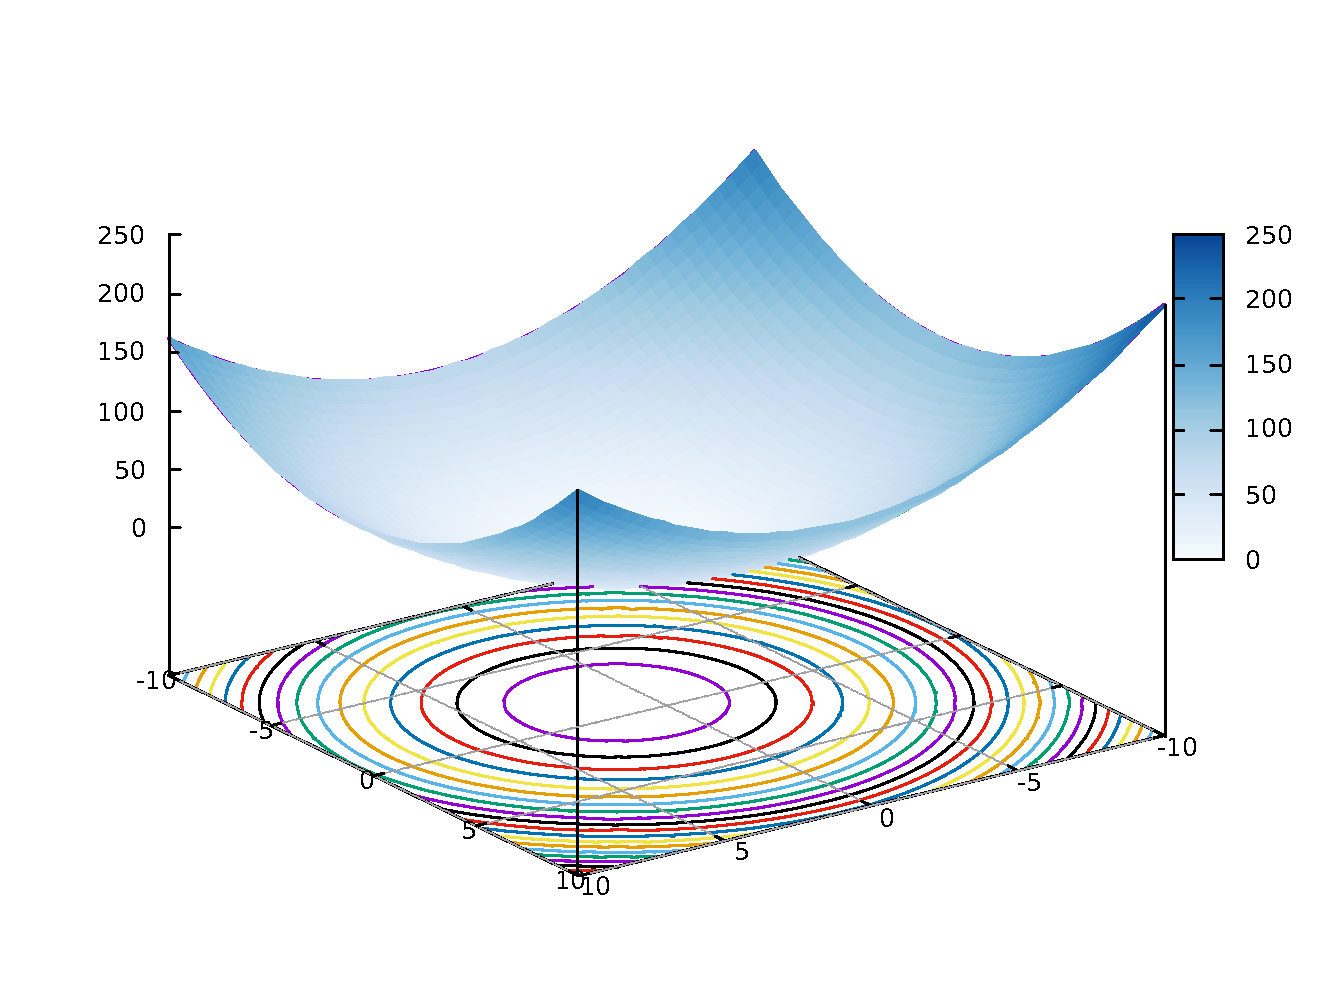
\includegraphics[width=1\columnwidth]{figures/numerical-methods-chemical-equilibrium/parabolic-plot}
\end{itemize}
\column{0.6\textwidth}

\vskip -10pt
\pause
\begin{itemize}
\item The values of $(x,y)$ that minimizes $f$ can be found using:
\begin{alignat*}{3}
\frac{\partial f}{\partial x} & =0 \; & \implies & \; & 2(x-1) & = 0 \; \implies  \; x = 1\\
\frac{\partial f}{\partial y} & =0 & \implies &  & 2(y+1) & =0 \; \implies  \; y = -1.
\end{alignat*}
\pause
%\begin{itemize}
\item \alert{\textbf{Question}}: How can we tell, mathematically, that the solution
above corresponds to a minimum?
\begin{center}
	\href{http://etc.ch/cKvh}{\textcolor{indigo(dye)}{\tt http://etc.ch/cKvh}} \quad or \quad 
	
\includegraphics[height=0.15\columnwidth]{figures/numerical-methods-chemical-equilibrium/polls.png}
\end{center}
\hiddenpause
\vskip 5pt
\item \textbf{Answer:} Check if the derivatives $\partial^{2}f/\partial x^{2}$
and $\partial^{2}f/\partial y^{2}$ at $(1,-1)$ are non-negative.
%\end{itemize}
\end{itemize}
\end{columns}
\end{frame}
%
% --------------------------------------------------------------------------------------------------------------------%
% Distinguishing between minimum, maximum, saddle-point values
% --------------------------------------------------------------------------------------------------------------------%
%
\begin{frame}{Distinguishing between minimum, maximum, saddle point values}
\begin{itemize}
\item In general, one checks 
the \alert{\bf eigenvalues of Hessian matrix} 
\[
H=\begin{bmatrix}\dfrac{\partial^{2}f}{\partial x^{2}} & \dfrac{\partial^{2}f}{\partial x\partial y}\\
\dfrac{\partial^{2}f}{\partial y\partial x} & \dfrac{\partial^{2}f}{\partial y^{2}}
\end{bmatrix}
\]
at obtained stationary point $(x_\star, y_\star)$.
%
\item If {\bf the eigenvalues are non-negative} at the $(x_\star, y_\star)$ (or Hessian is a positive semi-definite matrix at $(x_\star, y_\star)$), this point is indeed a {\bf local minimum}.
%
\item If {\bf the eigenvalues are negative} at the $(x_\star, y_\star)$ (or Hessian is negative-definite at $(x_\star, y_\star)$), this  point is a {\bf local maximum}.
%
\item If {\bf the eigenvalues are of different signs} at the $(x_\star, y_\star)$, this point is a {\bf saddle point}.
\end{itemize}
\end{frame}
%
% --------------------------------------------------------------------------------------------------------------------%
% Example of saddle point problem
% --------------------------------------------------------------------------------------------------------------------%
%
	\begin{frame}{Example of saddle point problem}
	\begin{columns}[t]
	
	\column{0.5\textwidth}
	\begin{itemize}
	\item Consider the function $f$ defined as:
	\[
	f(x,y)=x^{2}-y^{2}.
	\]
	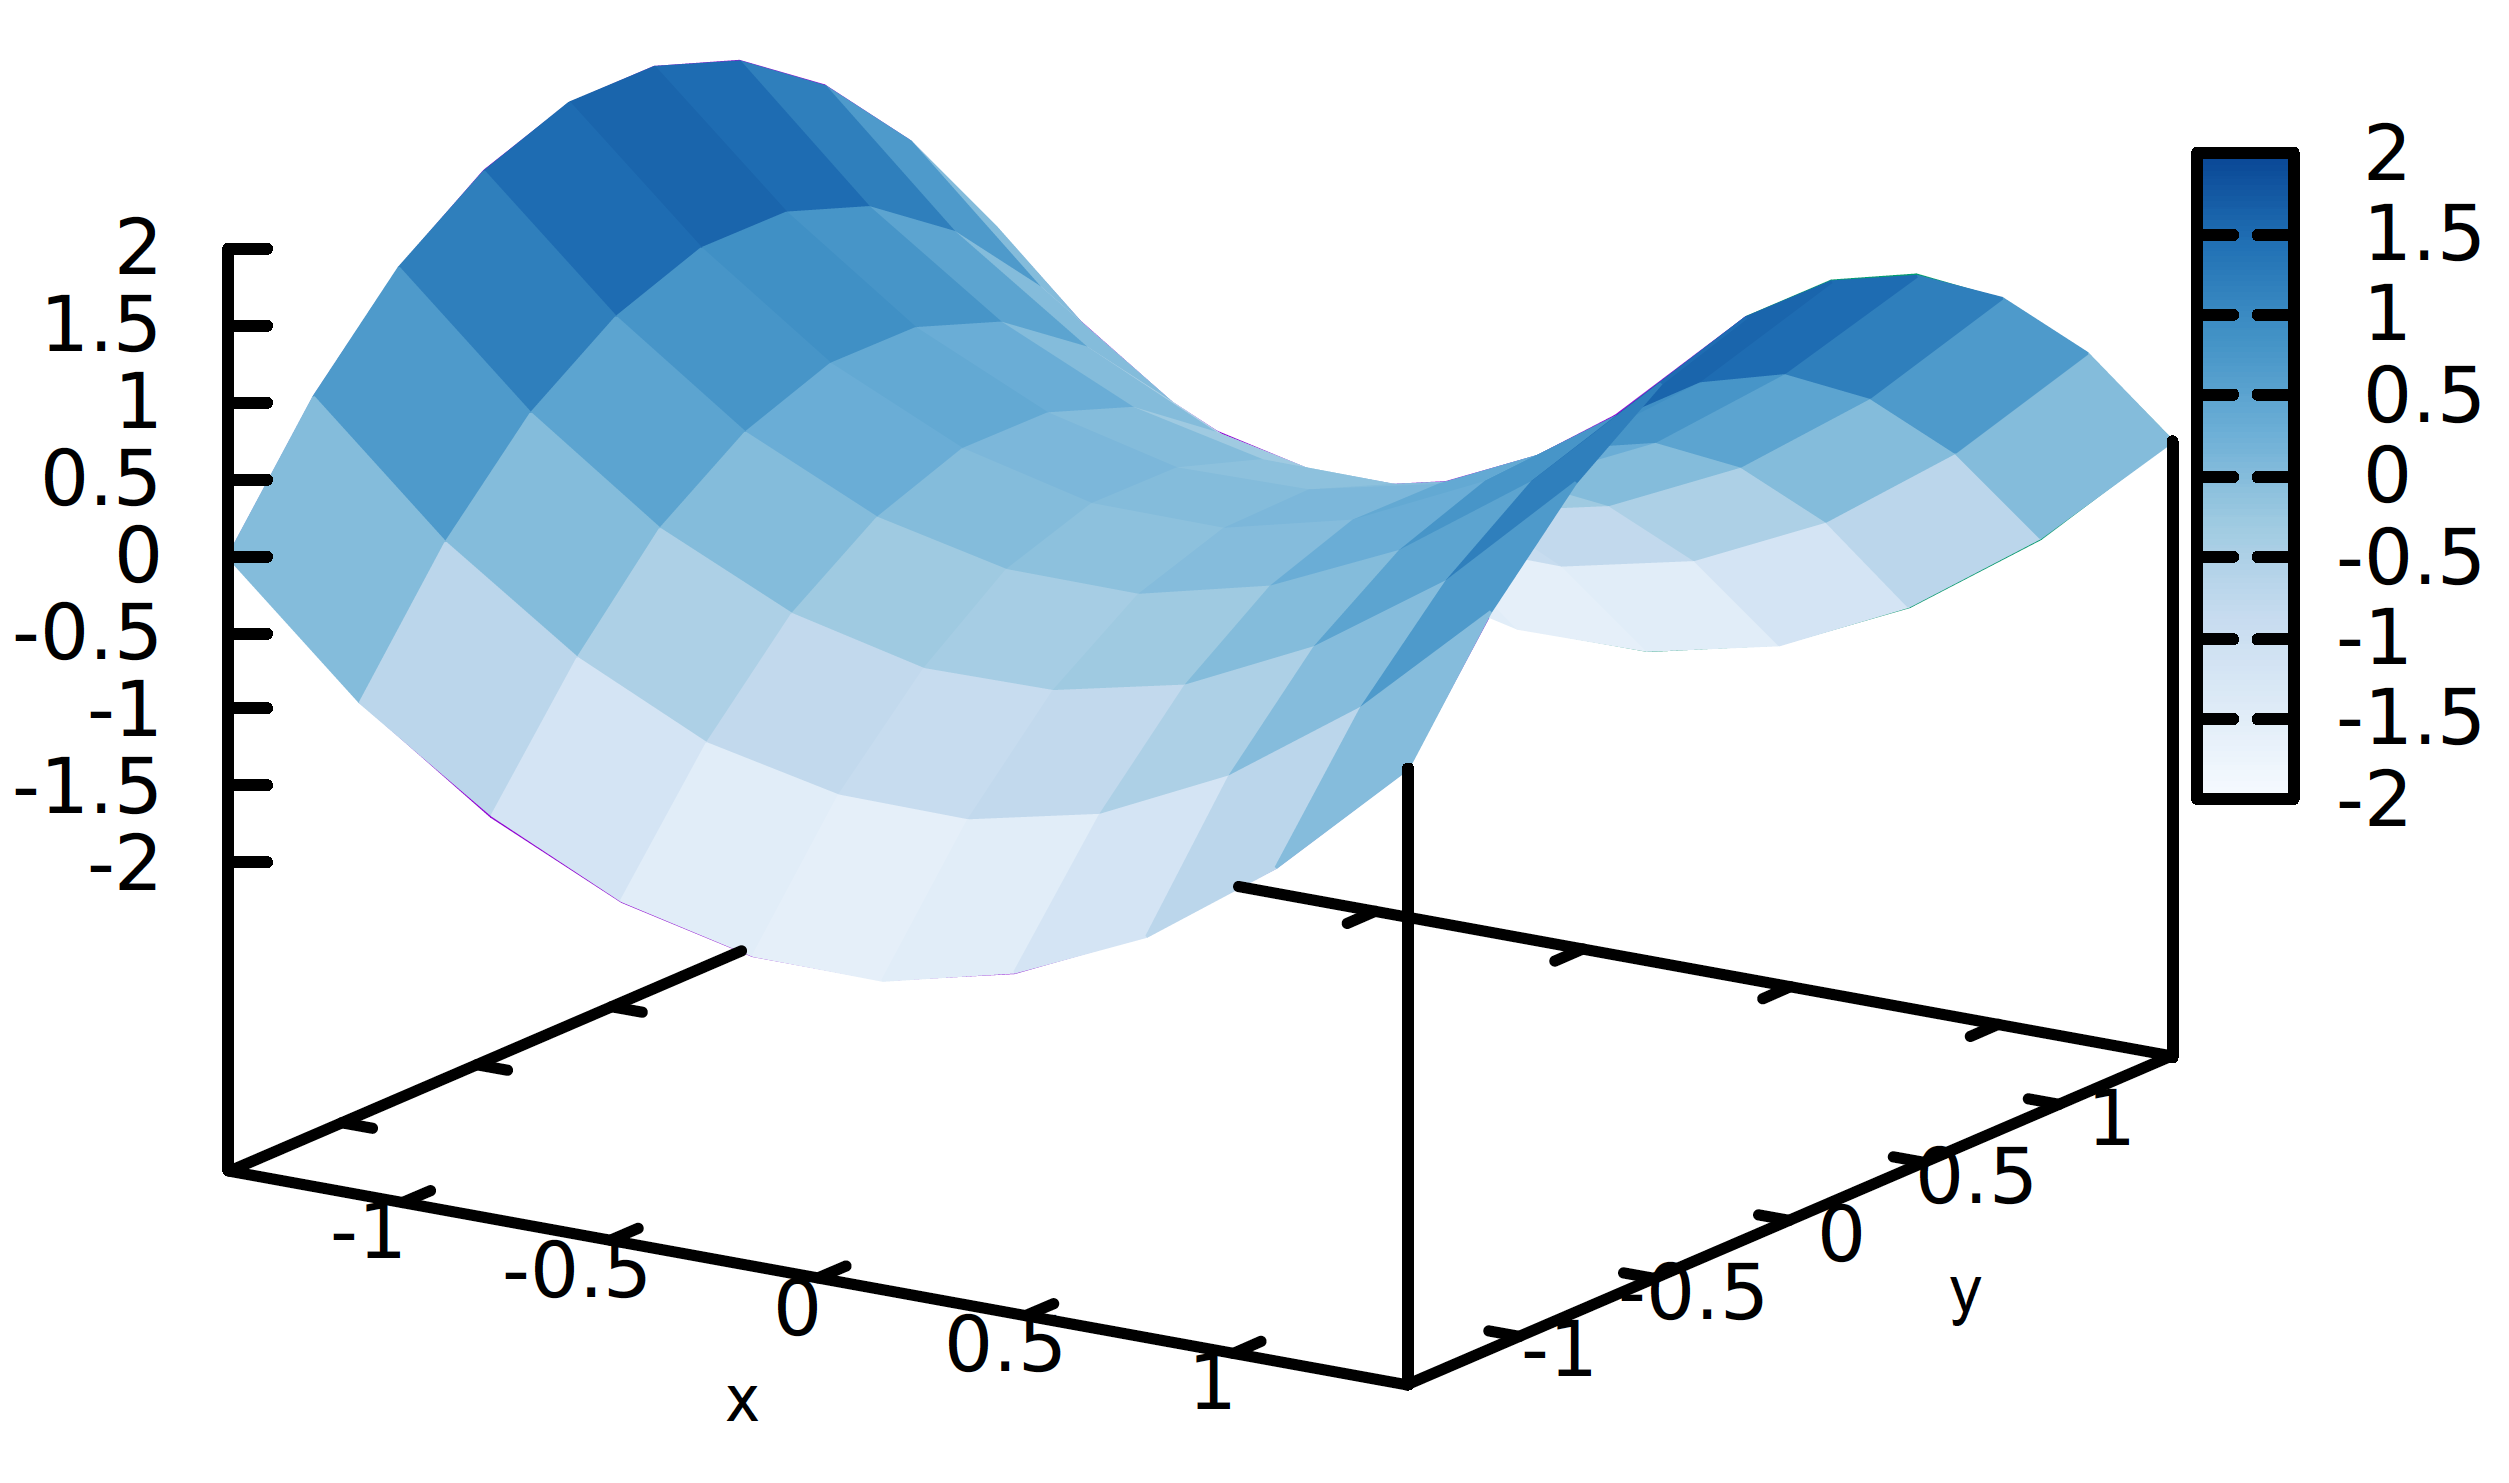
\includegraphics[width=1\columnwidth]{figures/numerical-methods-chemical-equilibrium/saddle-point-with-axis.png}
	\end{itemize}
	
	\column{0.5\textwidth}
	\pause
	\begin{itemize}
	\item At $(x,y)=(0,0)$: 
	\[
	{\displaystyle \frac{\partial f}{\partial x}=\frac{\partial f}{\partial y}=0,}
	\]
	but $f(0,0)=0$ is \textbf{neither a minimum nor a maximum}. 
	%
	\pause
	\item \alert{\textbf{Quiz:}} What are the signs of $\partial^{2}f/\partial x^{2}$ and $\partial^{2}f/\partial y^{2}$ for this example?
	%
	\begin{center}
		\href{http://etc.ch/cKvh}{\textcolor{indigo(dye)}{\tt http://etc.ch/cKvh}} \quad or \quad 
		
\includegraphics[height=0.15\columnwidth]{figures/numerical-methods-chemical-equilibrium/polls.png}
	\end{center}
	%
	\hiddenpause
	\item {\textbf{Answer:}} The values of $\partial^{2}f/\partial x^{2}>0$
	and $\partial^{2}f/\partial y^{2}<0$ at $(0,0)$, which implies a \alert{\bf saddle point}.
	\end{itemize}
	\end{columns}
	
	\end{frame}
%
% --------------------------------------------------------------------------------------------------------------------%
% Lagrangian function of chemical equilibrium problem 
% --------------------------------------------------------------------------------------------------------------------%
\subsection{Constrained minimization}
%
\begin{frame}{Lagrangian function of chemical equilibrium problem}
\begin{itemize}
\item Because of the {\bf mass conservation constraints}, $An=b$, and
the {\bf non-negative constraints}, $n\geq0$, we need to write
the \alert{\textbf{Lagrange function}} $L$ for the Gibbs energy minimization problem:
\[
L(n,y,z):=G(n)-(An-b)^{T}y-n^{T}z,
\]
where the \alert{unknowns} $n$, $y$, and $z$ correspond to
%
\begin{itemize}
\item the vector of \emph{species amounts} $n=(n_{1},\ldots,n_{\text{N}})$, 
\item the vector of \emph{Lagrange multipliers} $y=(y_{1},\ldots,y_{\text{E}})$, and 
\item the vector of \emph{complementary variables} $z=(z_{1},\ldots,z_{\text{N}})$ that satisfy 
%	
\[
n_{i}\, z_{i}=0,\qquad n_{i}\geq0,\qquad z_{i}\geq0.
\]
\end{itemize}
\pause
\item {\bf Note}: The above form of the Lagrangian function is called {\bf matrix form} but one can write it explicitly for each unknown $n_{i}$, $y_{j}$, and $z_{i}$. 
\end{itemize}
\end{frame}
%
% --------------------------------------------------------------------------------------------------------------------%
% System of equation corresponding to minimization of Lagrangian
% --------------------------------------------------------------------------------------------------------------------%
%
\begin{frame}{System of equation corresponding to minimization of Lagrangian}
\begin{itemize}
\item Instead of finding \alert{only} $n=(n_{1},\ldots,n_{\text{N}})$ that solves 
\begin{alignat*}{2}
\frac{\partial G}{\partial n_{i}} & =0 & \qquad & (i=1,\ldots,\text{N}),
\end{alignat*}
\pause
 we find \alert{$n=(n_{1},\ldots,n_{\text{N}})$}, \alert{$y=(y_{1},\ldots,y_{\text{E}})$},
and \alert{$z=(z_{1},\ldots,z_{\text{N}})$} that solves 
\begin{alignat*}{2}
\frac{\partial L}{\partial n_{i}} & =0 & \qquad\vphantom{\frac{\partial L}{\partial y_{j}}} & (i=1,\ldots,\text{N}),\\
\frac{\partial L}{\partial y_{j}} & =0 & \vphantom{\frac{\partial L}{\partial y_{j}}} & (j=1,\ldots,\text{E}),\\
n_{i}z_{i} & =0 & \vphantom{\frac{\partial L}{\partial y_{j}}} & (i=1,\ldots,\text{N}),\\
n_{i},z_{i} & \geq0 & \vphantom{\frac{\partial L}{\partial y_{j}}} & (i=1,\ldots,\text{N}).
\end{alignat*}
\end{itemize}
\end{frame}
%
% --------------------------------------------------------------------------------------------------------------------%
% System of equation corresponding to minimization of Lagrangian \, ii
% --------------------------------------------------------------------------------------------------------------------%
%
\begin{frame}{System of equation corresponding to minimization of Lagrangian \, ii}

\small
\begin{columns}[c]
%
\column{0.5\textwidth}
%
We rewrite the system of equations \\[10pt]
%
\begin{alignat*}{2}
\frac{\partial L}{\partial n_{i}} & =0 & \qquad\vphantom{\frac{\partial L}{\partial y_{j}}} & (i=1,\ldots,\text{N}),\\[10pt]
\frac{\partial L}{\partial y_{j}} & =0 & \vphantom{\frac{\partial L}{\partial y_{j}}} & (j=1,\ldots,\text{E}),\\
n_{i}z_{i} & =0 & \vphantom{\frac{\partial L}{\partial y_{j}}} & (i=1,\ldots,\text{N}),\\
n_{i},z_{i} & \geq0 & \vphantom{\frac{\partial L}{\partial y_{j}}} & (i=1,\ldots,\text{N}),
\end{alignat*}
\column{0.5\textwidth}
%
using the definition of $\mu_{i}\coloneqq\partial G/\partial n_{i}$: 
\pause
\begin{overprint}
\onslide<2-> 
\begin{alignat*}{2}
\mu_{i}-\sum_{j=1}^{\text{E}}A_{ji}y_{j} & -z_{i}=0 & \qquad\vphantom{\frac{\partial L}{\partial y_{j}}} & (i=1,\ldots,\text{N}),\\
\sum_{i=1}^{\text{N}}A_{ji}n_{i}-b_{j} & =0 & \vphantom{\frac{\partial L}{\partial y_{j}}} & (j=1,\ldots,\text{E}),\\
n_{i}z_{i} & =0 & \vphantom{\frac{\partial L}{\partial y_{j}}} & (i=1,\ldots,\text{N}),\\
n_{i},z_{i} & \geq0 & \vphantom{\frac{\partial L}{\partial y_{j}}} & (i=1,\ldots,\text{N}).
\end{alignat*}
\end{overprint}
\end{columns}
\pause
\vskip 10pt
\alert{\bf Note}: Since $\mu_{i}$ is a function of unknown $n_{i}$, we obtain {\bf non-linear system of equation}.

\end{frame}

\section{Interior-point method for constrained minimization}
%
% --------------------------------------------------------------------------------------------------------------------%
% General minimization formulation representing the GEM problem
% --------------------------------------------------------------------------------------------------------------------%
%
\begin{frame}{Abstract constrained minimization formulation}
	\small
\begin{itemize}
\item Solve the following general \alert{\bf constrained minimization problem}:
\[
\min_{x}f(x)\qquad\text{subject to}\qquad Ax=b\quad\text{and}\quad x\geq0.
\]
\vskip -10pt
\pause
\item \alert{\textbf{Quiz}}: What would be $f(x)$ and $x$ in a context of chemical equilibrium problem?
%
\begin{center}
	\href{http://etc.ch/cKvh}{\textcolor{indigo(dye)}{\tt http://etc.ch/cKvh}} \quad or \quad 
	
\includegraphics[height=0.13\columnwidth]{figures/numerical-methods-chemical-equilibrium/polls.png}
\end{center}
\hiddenpause
\item \alert{\textbf{Answer}}: We will define $f$ as our Gibbs energy function
\[
f(x)=G(x;T,P),
\]
\vskip -10pt
where 
\begin{itemize}
\item $x=(x_{1},\ldots,x_{\text{n}})$ represents the \alert{unknown
species amounts}, ${n=(n_{1},\ldots,n_{\text{N}})}$, 
\item $A$ specifies the \alert{formula matrix of the system}, and 
\item $b$ stands for the \alert{vector of element amounts}.
\end{itemize}
\end{itemize}
\end{frame}
%
% --------------------------------------------------------------------------------------------------------------------%
% Lagrangian of general minimization formulation
% --------------------------------------------------------------------------------------------------------------------%
%
\begin{frame}{Lagrangian of general minimization formulation}

\small
\begin{itemize}[<+->]
\item First, we write the {\bf Lagrange function for the general minimization problem}:
\[
L(x,y,z)=f(x)-(Ax-b)^{T}y-x^{T}z.
\]
\item Then, we formulate its \textbf{first-order necessary conditions for the minimum}:
%
\begin{alignat*}{2}
\partial f/\partial x-A^{T}y-z & =0, & \qquad\\
Ax-b & =0,\\
x_{i}z_{i} & =0 &  & (i=1,\ldots,n),\\
x_{i},z_{i} & \geq0 &  & (i=1,\ldots,n).
\end{alignat*}
%
%where $g=\partial f/\partial x$.
\end{itemize}
\end{frame}
%
% --------------------------------------------------------------------------------------------------------------------%
% Complementarity conditions
% --------------------------------------------------------------------------------------------------------------------%
%
\begin{frame}{Complementarity conditions}

%\lcol
\begin{itemize}
\item The \alert{\bf complementarity conditions}
\begin{align*}
x_{i}z_{i} & =0\\
x_{i} & \geq0\\
z_{i} & \geq0
\end{align*}
 are {\bf challenging to solve numerically}.
%\rcol
\item They are sharp conditions, in which
\begin{alignat*}{3}
x_{i} & \geq0 & \qquad\text{and}\qquad & z_{i} & =0\\
\shortintertext{or}x_{i} & =0 & \qquad\text{and}\qquad & z_{i} & \geq0.
\end{alignat*}
%\item \textbf{Question:} What is the value of $\partial x_{i}/\partial z_{i}$
%when 
%\begin{itemize}
%\item $x_{i}=0$ and $z_{i}\geq0$?
%\item $x_{i}\geq0$ and $z_{i}=0$?
%\end{itemize}

\end{itemize}
%\ecol
\end{frame}
%
% --------------------------------------------------------------------------------------------------------------------%
% Interior-point perturbation approach
% --------------------------------------------------------------------------------------------------------------------%
\subsection{Interior-point perturbation approach}
%
\begin{frame}{Interior-point perturbation approach}
\small 
\lcol
\begin{itemize}
\item Perturb $x_{i}z_{i}=0$ with a \alert{\textbf{small and constant number}}
%
\[
x_{i}z_{i}=\tau.
\]
\item \textbf{Note:} the choice of $\tau$ affects the smallest amount a
species that can exist in equilibrium. 
\item \textbf{Example:} the choice $\tau=10^{-20}$ causes species in
\textbf{unstable phases} to have amounts around this value.  
\end{itemize}
\rcol

\begin{figure}
\centering{}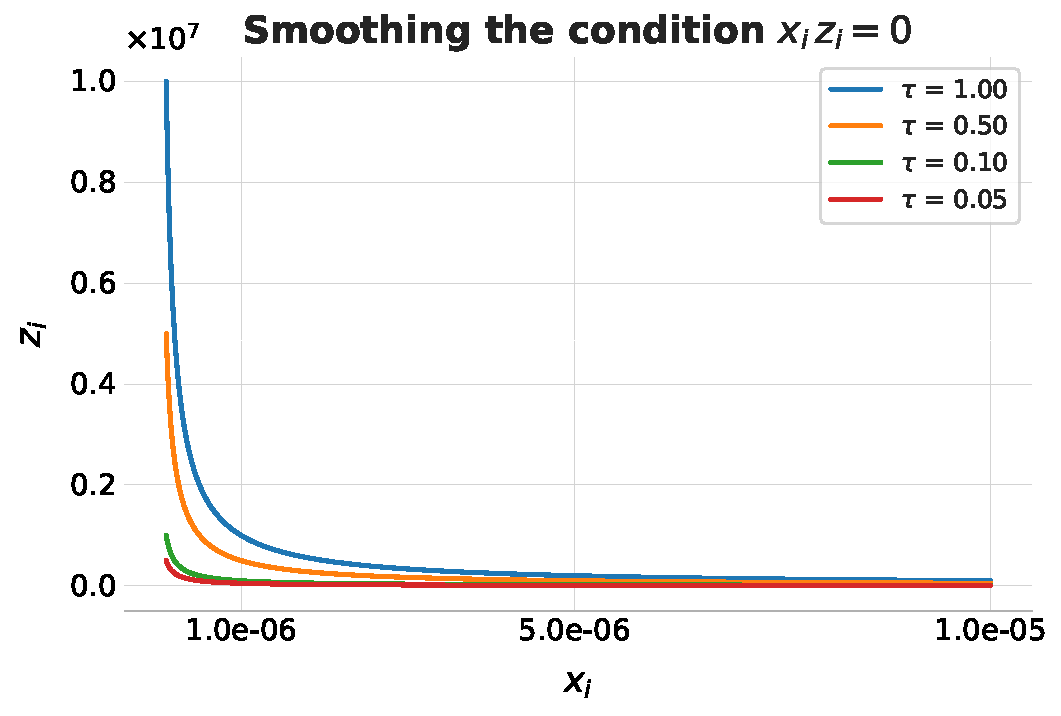
\includegraphics[width=0.8\columnwidth]{figures/numerical-methods-chemical-equilibrium/smoothing-complementarity-condition}
\end{figure}

\ecol

\begin{itemize}
	\item \alert{\bf Quiz}: What can we say about the amount of mineral dissolved in water?
	%
	\begin{center}
		\href{http://etc.ch/cKvh}{\textcolor{indigo(dye)}{\tt http://etc.ch/cKvh}} \quad or \quad 
		
\includegraphics[height=0.1\columnwidth]{figures/numerical-methods-chemical-equilibrium/polls.png}
	\end{center}
	\hiddenpause
	\item \alert{\bf Answer}: The amount will be of order $\tau$.
\end{itemize}
\end{frame}
%
% --------------------------------------------------------------------------------------------------------------------%
% Interior-point Newton method
% --------------------------------------------------------------------------------------------------------------------%
%
\begin{frame}{Interior-point Newton method}
\begin{columns}[t]

\column{0.5\textwidth}
\begin{itemize}
\item We'll use \alert{\bf Newton's method} to solve 
the obtained system of non-linear equations:
%
\begin{alignat*}{2}
\frac{\partial f}{\partial x} - A^{T}y-z & =0, & \qquad\\
Ax-b & =0,\\
x_{i}z_{i} & =\tau &  & (i=1,\ldots,n),\\
x_{i},z_{i} & \geq0 &  & (i=1,\ldots,n).
\end{alignat*}
%
%where $g(x) = \partial f / \partial x$.
\end{itemize}

\column{0.5\textwidth}
\begin{itemize}
\item Define the \alert{\bf residual function} $F$ as follows:
\[
F(x,y,z)\coloneqq
%\begin{bmatrix}F_{1}\\
%F_{2}\\
%F_{3}
%\end{bmatrix}
\begin{bmatrix}
\frac{\partial f}{\partial x} - A^{T}\,y-z\\
Ax-b\\
XZe-\tau
\end{bmatrix}, 
\]
%
where 
\begin{itemize}
\item $e=(1,\ldots,1)^{T}$,
\item $X=\text{diag}(x)$, and 
\item $Z=\text{diag}(z)$.
\end{itemize}
\end{itemize}
\end{columns}
\vskip 10pt
\begin{tcolorbox}
	The resulting problem: find $(x,y,z)$, with $x,z\geq0$, so that: 
	\[
	F(x,y,z)=0.
	\]
\end{tcolorbox}

\end{frame}
%
% --------------------------------------------------------------------------------------------------------------------%
% Jacobian matrix for the interior-point Newton method
% --------------------------------------------------------------------------------------------------------------------%
%
% TODO : either solve the issue with items, \pause, and \onslide or separate this slide to two!
\begin{frame}{Jacobian matrix for the interior-point Newton method}
%
\lcol
\begin{itemize}
\item Newton's method require the Jacobian $J$ of the residual function:
\[
F(x,y,z)
%\coloneqq
%\begin{bmatrix}
%F_{1}\\
%F_{2}\\
%F_{3}
%\end{bmatrix}
\coloneqq\begin{bmatrix}
\frac{\partial f}{\partial x}-A^{T}y-z\\
Ax-b\\
XZe-\tau
\end{bmatrix},
\]
which is defined as  
\[
J :=\begin{bmatrix}
\frac{\partial F_1}{\partial x} & \frac{\partial F_1}{\partial y} & \frac{\partial F_1}{\partial z}\\
\frac{\partial F_2}{\partial x} & \frac{\partial F_2}{\partial y} & \frac{\partial F_2}{\partial z}\\
\frac{\partial F_3}{\partial x} & \frac{\partial F_3}{\partial y} &\frac{\partial F_3}{\partial z}
\end{bmatrix}.
\]
%
\pause
\item \alert{\textbf{Exercise}}: derive the matrix blocks in Jacobian of $J$.
\end{itemize}
\rcol
\hiddenpause
\begin{itemize}
	\item {\bf Answer}:
	\[
	J
	=\begin{bmatrix}
			H & -A^{T} & -I\\
			A & 0 & 0\\
			Z & 0 & X
		\end{bmatrix}.
	\]
where 
\begin{itemize}
	\item $I$ be the identity matrix and
	%
	\item $H$ represent the Hessian matrix of $f$ (second derivatives of $f$)
	%
	\[
	H :=
	%\frac{\partial g}{\partial x}=
	\frac{\partial^{2}f}{\partial x^{2}}.
	\]
\end{itemize}
%
\pause
\item \alert{\bf How can we calculate Hessian matrix $H$?}
\end{itemize}

\ecol
\end{frame}
%
\subsection{Hessian matrix of the Gibbs energy function}
%
% --------------------------------------------------------------------------------------------------------------------%
% Hessian matrix of the Gibbs energy function
% --------------------------------------------------------------------------------------------------------------------%
\begin{frame}{Hessian matrix of the Gibbs energy function}
\begin{itemize}
\item The \alert{\bf Hessian matrix of the Gibbs energy} is
\[
H :=\frac{\partial^{2}G}{\partial n^{2}} 
\qquad\text{or in element-wise notation}\qquad 
H :=\big\{ H_{ij} \big\}_{ij} 
:= \Bigg\{ \frac{\partial^{2}G}{\partial n_{i}\partial n_{j}}\Bigg\}_{ij} 
\]
\item Recall that
\[
\frac{\partial G}{\partial n_{i}}=\mu_{i}\qquad\text{and}\qquad\mu_{i}=\mu_{i}^{\circ}+RT\ln a_{i}.
\]
\item Thus, 
\[
H_{ij}=\frac{\partial\mu_{i}}{\partial n_{j}}=\frac{\partial}{\partial n_{j}}\left(\mu_{i}^{\circ}+RT\ln a_{i}\right)=RT\frac{\partial\ln a_{i}}{\partial n_{j}}.
\]
\item Expressions for $\partial\ln a_{i}/\partial n_{j}$ can be derived
for all previous activity models.
\end{itemize}
\end{frame}
%
% --------------------------------------------------------------------------------------------------------------------%
% Partial molar derivatives of activities
% --------------------------------------------------------------------------------------------------------------------%
\begin{frame}{Partial molar derivatives of activities}
\begin{itemize}[<+->]
\item Instead of exact calculation of partial molar derivatives, 
we {\bf derive  them for ideal models}.
\item We use activity models to {\bf correct for the non-ideal behavior}
of the aqueous and gaseous solutions.
\item We use the partial molar derivatives of ideal activity models as it is {\bf simpler to derive}. 
%
\item So, in\\[-30pt]
%
\begin{alignat*}{2}
	\mu_{i}-\sum_{j=1}^{\text{E}}A_{ji}y_{j} & -z_{i}=0 & \qquad\vphantom{\frac{\partial L}{\partial y_{j}}} & (i=1,\ldots,\text{N}),\\[-10pt]
	\sum_{i=1}^{\text{N}}A_{ji}n_{i}-b_{j} & =0 & \vphantom{\frac{\partial L}{\partial y_{j}}} & (j=1,\ldots,\text{E}),\\[-15pt]
	n_{i}z_{i} & =0 & \vphantom{\frac{\partial L}{\partial y_{j}}} & (i=1,\ldots,\text{N}),\\[-10pt]
	n_{i},z_{i} & \geq0 & \vphantom{\frac{\partial L}{\partial y_{j}}} & (i=1,\ldots,\text{N}),
\end{alignat*}
%
\alert{\bf $\mu_{i}$ will be calculated exactly}. But the {\bf Jacobian will be approximated}.
%
\item Ideally, an \alert{\bf automatic differentiation} scheme should be used
to compute these derivatives (beyond the scope of this course).
\end{itemize}

\end{frame}
%
% --------------------------------------------------------------------------------------------------------------------%
% Partial molar derivatives of activities -- aqueous solutes
% --------------------------------------------------------------------------------------------------------------------%
%
\begin{frame}{Partial molar derivatives of activities of aqueous solutes}
\begin{itemize}
\item Recall that the {\bf activity of an aqueous solute} is
\[
a_{i}=\gamma_{i}m_{i},\text{ where }m_{i}=55.508\frac{n_{i}}{n_{w}}.
\]
\pause
\item Its ideal activity model is $a_{i}=m_{i}$, with $\gamma_{i}=1$.
\hiddenpause
\item Thus, 
%
\begin{alignat*}{2}
\frac{\partial\ln a_{i}}{\partial n_{j}}
\approx\frac{\partial\ln m_{i}}{\partial n_{j}} 
& = \mathsf{\alert{Exercise}} \\
& \onslide<4->{
	= \frac{\partial55.508}{\partial n_j} 
   + \frac{\partial\ln n_{i}}{\partial n_{j}}
   - \frac{\partial\ln n_{w}}{\partial n_{j}}
         = \begin{cases}
         	\dfrac{1}{n_{i}} & j=i,\\
         	-\dfrac{1}{n_{w}} & j=w,\\
         	0 & \text{otherwise}.
         \end{cases}}
\end{alignat*}
\end{itemize}
\end{frame}
%
%\begin{frame}{Partial molar derivatives of activities -- aqueous solutes \, ii}
%\[
%\frac{\partial\ln a_{i}}{\partial n_{j}}\approx\frac{\partial\ln m_{i}}{\partial n_{j}}=\frac{\partial55.508}{\partial n_{j}}+\frac{\partial\ln n_{i}}{\partial n_{j}}-\frac{\partial\ln n_{w}}{\partial n_{j}
%}=\begin{cases}
%\dfrac{1}{n_{i}} & j=i\\
%-\dfrac{1}{n_{w}} & j=w\vphantom{^{^{^{^{^{^{^{^{^ {}}}}}}}}}}\\
%0 & \text{otherwise}\vphantom{^{^{^{^{^{^{^{^{^ {}}}}}}}}}}
%\end{cases}.
%\]
%\end{frame}
%
% --------------------------------------------------------------------------------------------------------------------%
% Partial molar derivatives of activities -- aqueous solvent, H2O(aq)
% --------------------------------------------------------------------------------------------------------------------%
%
\begin{frame}{Partial molar derivatives of activities of aqueous solvent, H$_{\boldsymbol{2}}$O(aq)}
%
\begin{itemize}
\item Recall that the {\bf ideal activity of water}, H$_{2}$O(aq), is
\[
a_{w}=-\frac{1-x_{w}}{x_{w}}, \qquad \text{where} \qquad 
x_{w}=\frac{n_{w}}{\sum n_{i}}.
\]
\hiddenpause
\item Thus, 
%
\begin{alignat*}{2}
\frac{\partial\ln a_{w}}{\partial n_{j}} & =\mathsf{\alert{Exercise}} \\
%
& \onslide<3->{= \frac{\partial\ln(x_{w}-1)}{\partial n_{j}}-\frac{\partial\ln x_{w}}{\partial n_{j}}=\begin{cases}
	-\dfrac{1}{n_{w}} & j=w,\\
	-\dfrac{1}{n_{w}}\dfrac{x_{w}}{x_{w}-1} \qquad \qquad & j\neq w.
\end{cases}}
\end{alignat*}
%
\end{itemize}

\end{frame}
%
% --------------------------------------------------------------------------------------------------------------------%
% Partial molar derivatives of activities -- aqueous solvent, H2O(aq) \, ii
% --------------------------------------------------------------------------------------------------------------------%
%
%\begin{frame}{Partial molar derivatives of activities — aqueous solvent, H$_{\boldsymbol{2}}$O(aq) \, ii}
%
%\[
%\frac{\partial\ln a_{w}}{\partial n_{j}}\approx
%\frac{\partial\ln(x_{w}-1)}{\partial n_{j}}-\frac{\partial\ln x_{w}}{\partial n_{j}}=\begin{cases}
%-\dfrac{1}{n_{w}} & j=w\\
%-\dfrac{1}{n_{w}}\dfrac{x_{w}}{x_{w}-1} & j\neq w\vphantom{^{^{^{^{^{^{^{^{^ {}}}}}}}}}}
%\end{cases}.
%\]
%
%\end{frame}
%
% --------------------------------------------------------------------------------------------------------------------%
% Partial molar derivatives of activities -- CO2(aq)
% --------------------------------------------------------------------------------------------------------------------%
%
\begin{frame}{Partial molar derivatives of activities of CO$_{\boldsymbol{2}}$(g)}

%\lcol
\vskip 10pt
\begin{itemize}
\item Recall that the {\bf activity of CO$_{2}$(g)} was calculated using
%
\[
a_{\mathsf{CO_{2}\text{(g)}}}=\varphi_{\mathsf{CO_{2}\text{(g)}}}\frac{P}{P^{\circ}},
\]
%
where the fugacity coefficient $\varphi_{\mathsf{CO_{2}\text{(g)}}}$
was only a function of $T$ and $P$, i.e., 
\[
\varphi_{\mathsf{CO_{2}\text{(g)}}}=\varphi_{\mathsf{CO_{2}\text{(g)}}}(T,P).
\]
\end{itemize}
%\rcol
\begin{itemize}
\hiddenpause
\item Thus, the value of the following derivative
%
\begin{alignat*}{2}
\frac{\partial\ln a_{\mathsf{CO_{2}\text{(g)}}}}{\partial n_{j}} & =\mathsf{\alert{Exercise}} \\
&\onslide<3->{ = 0.}
\end{alignat*}
%\item \textbf{Answer:}
%\[
%\frac{\partial\ln a_{\mathsf{CO_{2}\text{(g)}}}}{\partial n_{j}}=0.
%\]
\end{itemize}
%\ecol
\end{frame}
%
% --------------------------------------------------------------------------------------------------------------------%
% Partial molar derivatives of activities --  pure minerals
% --------------------------------------------------------------------------------------------------------------------%
%
\begin{frame}{Partial molar derivatives of activities -- pure minerals}
\begin{itemize}
\item Recall that the {\bf activities of pure minerals} 
(e.g., mineral phases with only one mineral end-member),
\[
a_{i}=1.
\]
\item Thus, for mineral species, 
\[
\frac{\partial\ln a_{i}}{\partial n_{j}}=0.
\]
\end{itemize}
\end{frame}
%
% --------------------------------------------------------------------------------------------------------------------%
% Calculation of the Hessian matrix of the Gibbs energy function in Python 
% --------------------------------------------------------------------------------------------------------------------%
%
\begin{frame}[fragile,allowframebreaks]{Calculation of the Hessian matrix of the Gibbs energy function in Python}
\begin{itemize}
\item Have a look in the Python code of the project to see the implementation
of these formulas for when calculating the Hessian matrix $H$ with
entry $H_{ij}$ given by:
\[
H_{ij}=RT\frac{\partial\ln a_{i}}{\partial n_{j}} 
\quad
\mbox{used in}
\quad
J=\begin{bmatrix}
	H & -A^{T} & -I\\
	A & 0 & 0\\
	Z & 0 & X
\end{bmatrix}.
\]
\end{itemize}

\begin{lstlisting}[language=Python, caption=Calculating Jacobian using Python]
# Define the function that calculates:
#  - G, the Gibbs energy of the system;
#  - u, the gradient of the Gibbs energy, or chemical potentials of the species
#  - H, the Hessian of the Gibbs energy, or partial molar derivatives of activities
# These quantities are normalized by RT for numerical reasons.
def gibbs_energy(T, P, n):
	RT = R*T
	u = chemical_potentials(T, P, n)/RT
	H = chemical_potentials_ddn(T, P, n)/RT
	G = n.dot(u)/RT
	return G, u, H

# Define the function that calculates the partial molar derivatives of the
# chemical potentials of the species.
def chemical_potentials_ddn(T, P, n):
	return R*T*ln_activities_ddn(T, P, n)
	
# Define the function that calculates the partial molar derivatives of the
# ln activities of all species
def ln_activities_ddn(T, P, n):
	# Create an array with the entries in n corresponding to aqueous species
	n_aqueous = n[slice_aqueous]
	
	# The matrix with partial molar derivatives of the activities
	ln_a_ddn = zeros((num_species, num_species))
	
	ln_a_ddn[slice_aqueous, slice_aqueous] = ln_activities_aqueous_species_ddn(T, P, n_aqueous)
	
	return ln_a_ddn

# Define the function that calculates the activities of the aqueous species.
# Parameters:
#   - T is temperature in units of K
#   - P is pressure in units of Pa
#   - nphase is an array with the mole amounts of the aqueous species
# Return:
#   - an array with the ln activities of aqueous species
def ln_activities_aqueous_species_ddn(T, P, nphase):
	# The molar amount of H2O(l)
	nH2O = nphase[iH2O]
	
	# The mole fraction of H2O(l)
	xH2O = nH2O/sum(nphase)
	
	# Calculate the partial molar derivatives of the solute activities
	ddn = diag(1.0/nphase) 		 #  1/ni, j = i
	ddn[:, iH2O] = -1.0/nH2O	 # -1/nw, j = w
	
	# Calculate the partial molar derivatives of the solvent water activity
	ddn[iH2O, :] = -1.0/nH2O * xH2O/(xH2O - 1.0) 	# -1/nw, j = w
	ddn[iH2O, iH2O] = -1.0/nH2O								 		#  1/nw*xw/(xw -1), j<>w
	
	return ddn
\end{lstlisting}
% TODO: provide here the links! 
\end{frame}
%
% --------------------------------------------------------------------------------------------------------------------%
% Numerical solution by the interior-point Newton method
% --------------------------------------------------------------------------------------------------------------------%
\subsection{Numerical solution by the interior-point Newton method}
%
\begin{frame}{Numerical solution by the interior-point Newton method}
%\begin{columns}[t]

%\column{0.5\textwidth}
\alert{\bf Newton method algorithm} at step 1: 
%
\begin{itemize}
%\item We now know how to calculate $H$ in the Jacobian matrix
%%
%\[
%J=\part{\begin{bmatrix}}
%	H & -A^{T} & -I\\
%	A & 0 & 0\\
%	Z & 0 & X
%\end{bmatrix}
%\]
%%
%in the Newton method.
\item At the first Newton iteration, start with {\bf initial guess} \\
${x^{0}=(x_{1}^{0},\ldots,x_{\text{n}}^{0})}$,
${y^{0}=(y_{1}^{0},\ldots,y_{\text{m}}^{0})}$ and ${z^{0}=(z_{1}^{0},\ldots,z_{\text{n}}^{0})}$. 
\end{itemize}

%\column{0.5\textwidth}
\begin{itemize}
\item Compute ${x^{1}=(x_{1}^{1},\ldots,x_{\text{n}}^{1})}$, ${y^{1}=(y_{1}^{1},\ldots,y_{\text{m}}^{1})}$
and ${z^{1}=(z_{1}^{1},\ldots,z_{\text{n}}^{1})}$ using
\begin{align*}
x^{1} & =x^{0}+\alpha_{x}^{0}\Delta x^{0}\\
y^{1} & =y^{0}+\Delta y^{0}\\
z^{1} & =z^{0}+\alpha_{z}^{0}\Delta z^{0}
\end{align*}
where $\alpha_{x}$ and $\alpha_{z}$ are introduced parameters to ensure $x_{i}^{1}>0$ and $z_{i}^{1}>0$. 
\item How do we calculate variations 
$\Delta x^{0}$, $\Delta y^{0}$, $\Delta z^{0}$?
\end{itemize}
%\end{columns}

\end{frame}
%
% --------------------------------------------------------------------------------------------------------------------%
% Numerical solution by the interior-point Newton method
% --------------------------------------------------------------------------------------------------------------------%
%
\begin{frame}{Numerical solution by the interior-point Newton method \, ii}
\begin{itemize}
\item To calculate the Newton variations ${\Delta x^{0}=(\Delta x_{1}^{0},\ldots,\Delta x_{\text{n}}^{0})}$,
${\Delta y^{0}=(\Delta y_{1}^{0},\ldots,\Delta y_{\text{m}}^{0})}$
and ${\Delta z^{0}=(\Delta z_{1}^{0},\ldots,\Delta z_{\text{n}}^{0})}$,
we solve the matrix equation 
%
\[
\underset{J^{0}}{\underbrace{\begin{bmatrix}H^{0} & -A^{T} & -I\\
A & 0 & 0\\
Z^{0} & 0 & X^{0}
\end{bmatrix}}}\begin{bmatrix}\Delta x^{0}\\
\Delta y^{0}\\
\Delta z^{0}
\end{bmatrix}=-\underset{F^{0}}{\underbrace{\begin{bmatrix}g^{0}-A^{T}y^{0}-z^{0}\\
Ax^{0}-b\\
X^{0}Z^{0}e-\tau
\end{bmatrix}}}
\]
%
where $J^{0}$, $F^{0}$, $H^{0}$, $Z^{0}$, $X^{0}$ represent to evaluation of respective matrices using the values of $x$, $y$, $z$ at the 0th iteration, i.e., 
\begin{itemize}
	\item $J^{0} := J(x^0, y^0, z^0)$, 
	\item $F^{0} := F(x^0, y^0, z^0)$, etc.
\end{itemize}
%$J^{0} := J(x^0, y^0, z^0)$ and $F^{0} := F(x^0, y^0, z^0)$.
%
%\item Here, terms with superscript $0$, for example $H^{0}$ and $g^{0}$, means evaluation using the values of $x$, $y$, $z$ at the 0th iteration.
\end{itemize}
\end{frame}
%
% --------------------------------------------------------------------------------------------------------------------%
% Numerical solution by the interior-point Newton method
% --------------------------------------------------------------------------------------------------------------------%
%
\begin{frame}{Numerical solution by the interior-point Newton method \, iii}
%
\vskip 10pt
\alert{\bf Newton method algorithm} at the step $k+1$: 
%	
\begin{itemize}
\item The vector steps $\Delta x^{k}$, $\Delta y^{k}$,
$\Delta z^{k}$ at the iteration $k$ is calculated by 
%
\[
J^k \, 
\begin{bmatrix}
	\Delta x^{k}\\
	\Delta y^{k}\\
	\Delta z^{k}
\end{bmatrix}
=- F^k
\]
%
\item New approximations $x^{k+1}$, $y^{k+1}$,
$z^{k+1}$ is obtained by
\begin{align*}
x^{k+1} & =x^{k}+\alpha_{x}^{k}\Delta x^{k},\\
y^{k+1} & =y^{k}+\Delta y^{k},\\
z^{k+1} & =z^{k}+\alpha_{z}^{k}\Delta z^{k}.
\end{align*}
\item How do we calculate $\alpha_{x}^{k}$ and $\alpha_{z}^{k}$ 
reassuring positivity of $x_{i}^{k+1}$ and $z_{i}^{k+1}$?
\end{itemize}
\end{frame}
%
% --------------------------------------------------------------------------------------------------------------------%
% Numerical solution by the interior-point Newton method
% --------------------------------------------------------------------------------------------------------------------%
%
\begin{frame}{Numerical solution by the interior-point Newton method \, iv}
%\begin{columns}[t]

%\column{0.6\textwidth}
\begin{itemize}
\item Start with $\alpha_{x}^{k}\gets1$.
\item Check if 
\[
x_{i}^{k}+\Delta x_{i}^{k}\leq0 \quad \text{for} \quad i=1,\ldots, n
\]
%
\begin{itemize}
\item if so, ${\displaystyle \alpha_{x}^{k}\gets(\delta-1)\frac{x_{i}^{k}}{\Delta x_{i}^{k}},}$
where $\delta\in(0,1)$, e.g., $\delta=10^{-4}$;
\item otherwise, go to next component with index $i$.
\end{itemize}
\item It results into either 
%\begin{itemize}
%\item 
a \alert{\bf full Newton step} (for $\alpha_{x}^{k}=1$) or
%\item 
a \alert{\bf partial Newton step}  (for $\alpha_{x}^{k}<1$).
%\end{itemize}
%\end{itemize}

%\column{0.4\textwidth}
%\begin{itemize}
\item If for certain index $i$, parameter $\alpha_{x}^{k}<1$, then
%
\[
x_{i}^{k+1}=\delta x_{i}^{k},
\]
and for all other indices
% 
\[
x_{j}^{k+1}=x_{j}^{k}+\alpha_{x}^{k}\Delta x_{j}^{k}, \quad j=1,\ldots, n, j\neq i.
\]
\end{itemize}
%\end{columns}

\end{frame}
%
% --------------------------------------------------------------------------------------------------------------------%
% Numerical solution by the interior-point Newton method
% --------------------------------------------------------------------------------------------------------------------%
%
\begin{frame}{Numerical solution by the interior-point Newton method \, v}
%\begin{columns}[t]
%\column{0.5\textwidth}
\vskip 10pt
\alert{\bf Summary of the Newton method algorithm}: \\[5pt]

\begin{itemize} 
%
\item With initial guess $x^{0}$, $y^{0}$, and $z^{0}$, repeat
%
\begin{alignat*}{2}
x^{k+1} & =x^{k}+\alpha_{x}^{k}\Delta x^{k}\\
y^{k+1} & =y^{k}+\Delta y^{k} & \qquad & \text{iteration }k\\
z^{k+1} & =z^{k}+\alpha_{z}^{k}\Delta z^{k}
\end{alignat*}
%
%\column{0.5\textwidth}
%
until
\[
\|F^{k}\|_{\infty}=\|F(x^{k},y^{k},z^{k})\|_{\infty}<\epsilon_{\mathrm{tol}},
\]
where
% 
\begin{itemize} 
\item $\epsilon_{\text{tol}}=10^{-6}$ is {\bf selected tolerance} and \item the {\bf norm of a vector $v$} is defined by
%
$
\|v\|_{\infty}=\max(|v_{i}|).
$
\end{itemize} 

\end{itemize} 
%\end{columns}

\end{frame}
%
%\section{Computational project}
%%
%\begin{frame}{Quiz on standard potentials}
%	
%	\begin{itemize}
%		\item \alert{\textbf{Quiz:}} what can we do alternatively to taking reference values of mu0, if we want to find standard potentials for pressures and temperatures lying in between the reference values?
%		%
%		\begin{center}
%			\href{http://etc.ch/cKvh}{\textcolor{indigo(dye)}{\tt http://etc.ch/cKvh}} \quad or \quad 
%			
\includegraphics[height=0.2\columnwidth]{figures/numerical-methods-chemical-equilibrium/polls.png}
%		\end{center}
%		%
%		\hiddenpause
%		\vskip 10pt
%		\item {\textbf{Answer:}} we interpolate between neighboring values of standard potentials.   
%		
%	\end{itemize}
%\end{frame}
%%
%\begin{frame}{Quiz on variable of EquilibriumState providing information on the solubility}
%	
%	\begin{itemize}
%		\item \alert{\textbf{Quiz:}} out of all these properties stored in the class EquilibriumState, which one will tell us the solubility of gas or mineral? 
%		%
%		\begin{center}
%			\href{http://etc.ch/cKvh}{\textcolor{indigo(dye)}{\tt http://etc.ch/cKvh}} \quad or \quad 
%			
\includegraphics[height=0.2\columnwidth]{figures/numerical-methods-chemical-equilibrium/polls.png}
%		\end{center}
%		%
%		\hiddenpause
%		\vskip 10pt
%		\item {\textbf{Answer:}} to make sure that we reach its solubility point, to dissolve the {\bf maximum} amount of CO$_2$(g) in the brine.
%	\end{itemize}
%	
%\end{frame}
%%
%\begin{frame}{Quiz on adding NaCl into the recipe}
%	
%	\begin{itemize}
%		\item \alert{\textbf{Quiz:}} what does happen to the solubility of CO$_2$(g) if we add NaCl into the recipe?
%		%
%		\begin{center}
%			\href{http://etc.ch/cKvh}{\textcolor{indigo(dye)}{\tt http://etc.ch/cKvh}} \quad or \quad 
%			
\includegraphics[height=0.2\columnwidth]{figures/numerical-methods-chemical-equilibrium/polls.png}
%		\end{center}
%		%
%		\hiddenpause
%		\item {\textbf{Answer:}} it decreases, salting-out effect.
%	\end{itemize}
%	
%\end{frame}
%%
%\begin{frame}{Quiz on the amount of CO$_2$ amount}
%		
%		\begin{itemize}
%			\item \alert{\textbf{Quiz:}} why do we add so much initial CO$_2$(g)?
%			%
%			\begin{center}
%				\href{http://etc.ch/cKvh}{\textcolor{indigo(dye)}{\tt http://etc.ch/cKvh}} \quad or \quad 
%				
\includegraphics[height=0.2\columnwidth]{figures/numerical-methods-chemical-equilibrium/polls.png}
%			\end{center}
%			%
%			\hiddenpause
%			\vskip 10pt
%			\item {\textbf{Answer:}} to make sure that we reach its solubility point, to dissolve the {\bf maximum} amount of CO$_2$(g) in the brine.
%		\end{itemize}
%	
%\end{frame}
%\begin{frame}{Acidity of recipes}
%	\small
%	\begin{itemize}
%		\item Given three mixture: \\
%			\begin{itemize}
%				\item  {\bf Mixture 1} :  1kg of water, 0.6 mol of NaCl, 1 mol of calcite \\
%				\item  {\bf Mixture 2} :  1kg of water, 0.6 mol of NaCl, 1 mol of calcite, 5 mol of CO$_2$(g)\\
%				\item  {\bf Mixture 3} :  1kg of water, 5 mol of CO$_2$(g)\\
%			\end{itemize}
%		\item \alert{\textbf{Quiz:}} sort out these mixture w.r.t increasing acidity (decreasing pH).\\[5pt]
%		%
%		\begin{center}
%			\href{http://etc.ch/cKvh}{\textcolor{indigo(dye)}{\tt http://etc.ch/cKvh}} \quad or \quad 
%			
\includegraphics[height=0.18\columnwidth]{figures/numerical-methods-chemical-equilibrium/polls.png}
%		\end{center}
%		%
%		\hiddenpause
%		\vskip 10pt
%		\item {\textbf{Answer:}} 1, 2, 3 because \\
%		\begin{itemize}
%			\item pH (Mixture 1) $\approx$ 10 \\
%			\item pH (Mixture 2) $\approx$ 6 \\
%			\item pH (Mixture 3) $\approx$ 4 \\
%		\end{itemize}
%	\end{itemize}
%
%	%b = element_amounts(kgH2O=1, molCO2=0.0, molNaCl=0.6, molCaCO3=1.0) -> pH = 10 (alkaline) 
%	%b = element_amounts(kgH2O=1, molCO2=5.0, molNaCl=0.6, molCaCO3=1.0) -> pH = 6 (slightly acidic)
%	%b = element_amounts(kgH2O=1, molCO2=5.0, molNaCl=0.0, molCaCO3=0.0) -> pH = 3.9 (acidic)
%\end{frame}
%
%\begin{frame}{pH dependence on the added amount of added CO$_2$(g)}
%	\small
%	\begin{itemize}
%
%		\item \alert{\textbf{Quiz:}} what happens around the point of added CO$_2$(g) equal 0.8 mols?\\[5pt]
%		%
%		\begin{center}
%			\href{http://etc.ch/cKvh}{\textcolor{indigo(dye)}{\tt http://etc.ch/cKvh}} \quad or \quad 
%			
\includegraphics[height=0.18\columnwidth]{figures/numerical-methods-chemical-equilibrium/polls.png}
%		\end{center}
%		%
%		\hiddenpause
%		\vskip 10pt
%		\item {\textbf{Answer:}} we have reached the saturation point of CO$_2$(g) in water, i.e., the aqueous solution cannot dissolve more CO$_2$ gas.
%		\end{itemize}
%\end{frame}
%
%\begin{frame}{Calcite solubility dependence on the added CO$_2$(g)}
%	\small
%	\begin{itemize}
%		
%		\item \alert{\textbf{Quiz:}} what does this plato with dissolved calcite indicate? \\[5pt]
%		%
%		\begin{center}
%			\href{http://etc.ch/cKvh}{\textcolor{indigo(dye)}{\tt http://etc.ch/cKvh}} \quad or \quad 
%			
\includegraphics[height=0.18\columnwidth]{figures/numerical-methods-chemical-equilibrium/polls.png}
%		\end{center}
%		%
%		\hiddenpause
%		\vskip 10pt
%		\item {\textbf{Answer:}} we have reached the saturation point of CO$_2$(g) in water, which does not effect the solubility of calcite.
%	\end{itemize}
%\end{frame}